% -------------------------------------------------------------------------------------------------%
\chapter{TINJAUAN PUSTAKA}
\label{chap:2}
%--------------------------------------------------------------------------------------------------%

%--------------------------------------------------------------------------------------------------%
\section{Knowledge Graph}
\label{sec:knowledge-graph}
%--------------------------------------------------------------------------------------------------%

\textit{Knowledge graph} merupakan model data berbasis \textit{graph} yang menggambarkan entitas
dunia nyata dan hubungan antara entitas-entitas tersebut \citep{seth_2019}. Sebagai contoh, pada
\pic~\ref{fig:kg-description} dapat dilihat terdapat entitas-entitas yang ditandai dengan bentuk
lingkaran, dan hubungan antara entitas-entitas ditandai dengan bentuk anak panah. Pada gambar dapat
dilihat bahwa terdapat entitas "James" dan "Louvre" dan properti "has visited" yang mengarah dari
"James" ke "Louvre". Relasi tersebut dapat kita anggap sebagai sebuah pengetahuan yang dalam bahasa
manusia dapat dituliskan sebagai ``James pernah mengunjungi Louvre''. Model data seperti ini cocok
untuk menyimpan data dengan banyak jenis relasi antara entitas seperti pengetahuan umum,
dibandingkan dengan \textit{relational database} yang cocok untuk menyimpan data dengan relasi antar
entitas yang sudah diketahui dan terbatas.

\begin{figure}[H]
  \centering
  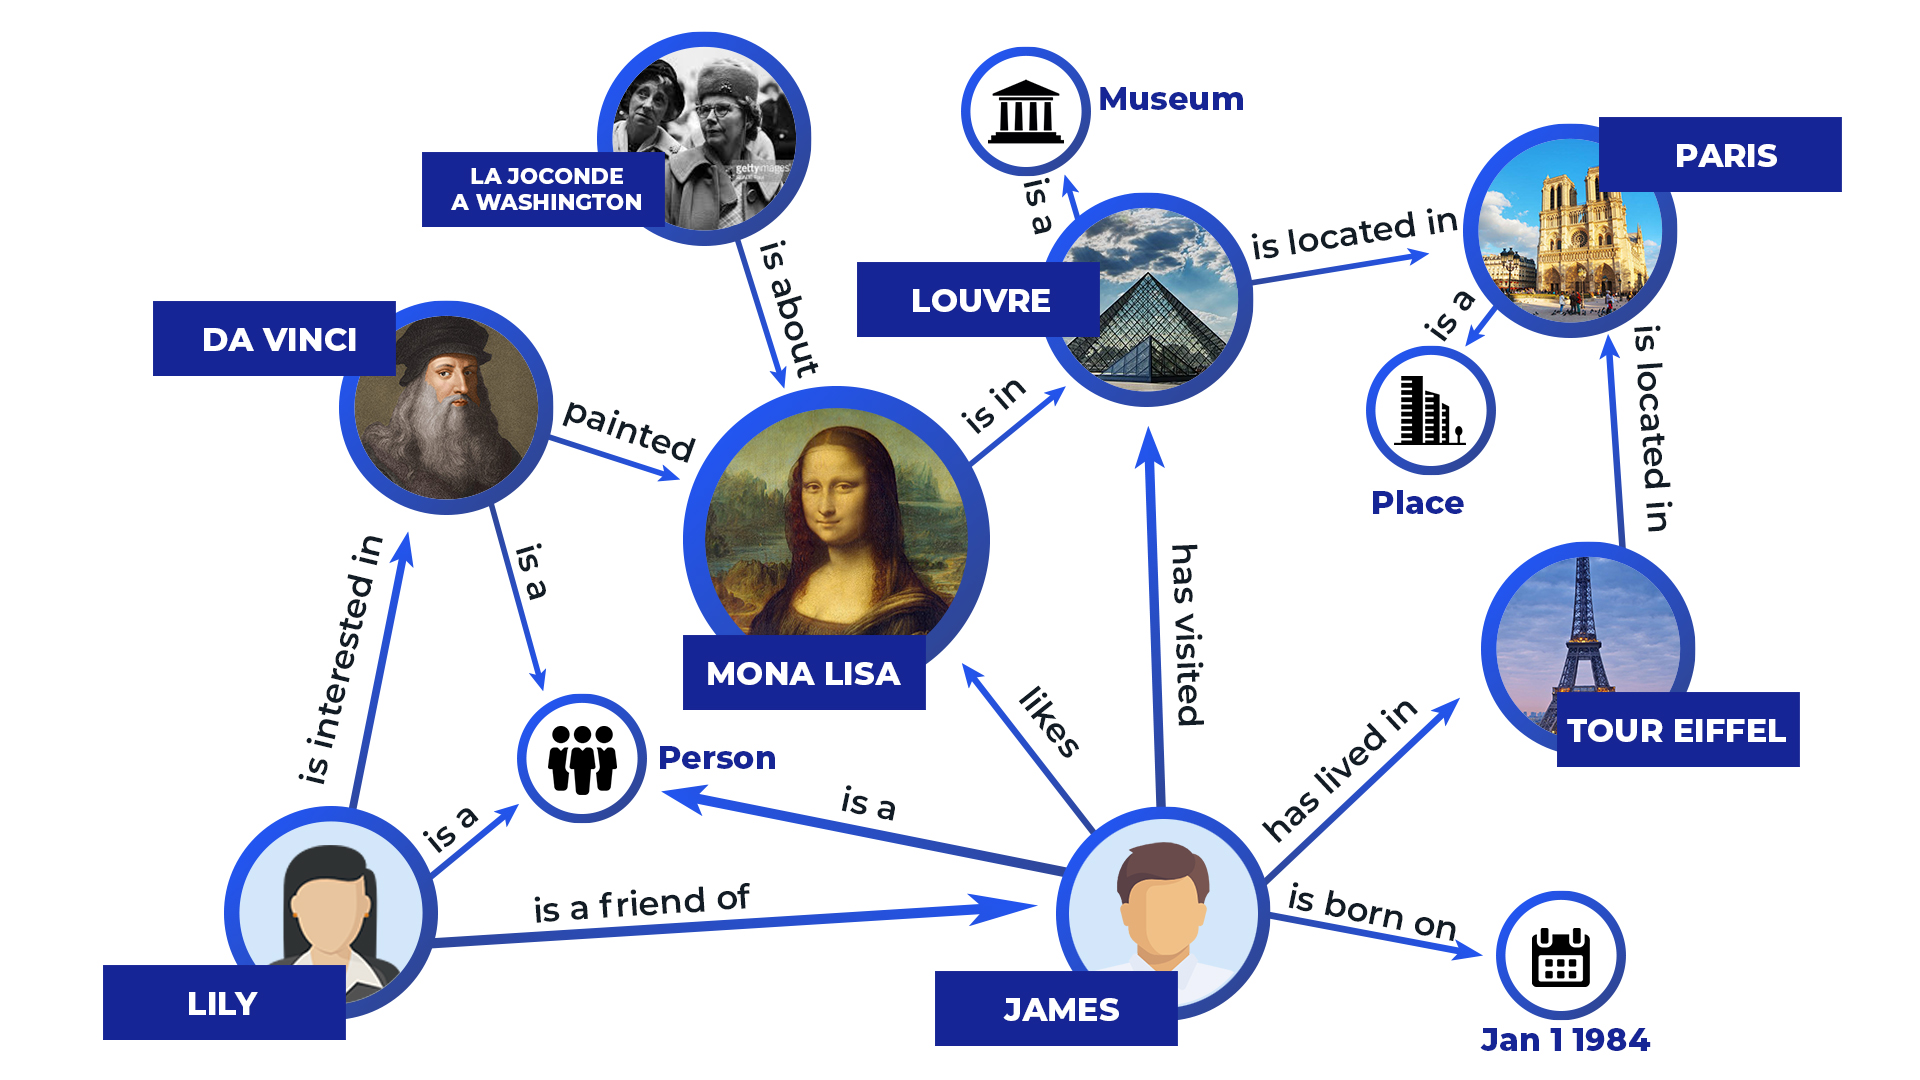
\includegraphics[width=\textwidth]{pictures/knowledge_graph.jpg}
  \caption[Contoh \textit{Knowledge Graph}]{Contoh \textit{Knowledge Graph}\\Sumber: \citep{seth_2019}}
  \label{fig:kg-description}
\end{figure}


%--------------------------------------------------------------------------------------------------%
\section{Resource Description Framework}
\label{sec:resource-description-framework}
%--------------------------------------------------------------------------------------------------%

Resource Description Framework (RDF) merupkan model data yang memberikan pernyataan tentang suatu
\textit{resource} dalam bentuk subjek-properti-objek, atau sering disebut \textit{triple}. Sebuah KG
dapat direpresentasikan sebagai kumpulan \textit{triple}. Subyek dan properti dalam \textit{triple}
direpresentasikan sebagai Uniform Resource Identifier (URI), sedangkan objek dapat direpresentasikan
dengan URI atau \textit{string literal}. Pada \pic~\ref{fig:triple-example}, dapat dilihat terdapat
KG dengan dua \textit{triple}. Pada \textit{Triple} 1, subjek, properti, dan objek berturut-turut
adalah \mono{https://example.org/James}, \mono{https://example.org/hasVisited},
\mono{https://example.org/Louvre} yang mana semuanya berbentuk URI. Sedangkan pada \textit{Triple}
2, subjek, properti, dan objek berturut-turut adalah \mono{https://example.org/James},
\mono{https://example.org/hasName}, "James". \mono{https://example.org/James},
\mono{https://example.org/Louvre} berturut-turut merupakan notasi untuk \textit{resource} entitas
James dan Louvre, \mono{https://example.org/hasVisited} dan \mono{https://example.org/hasName}
merupakan properti yang menjelaskan hubungan antara subjek dan objek, dan "James" adalah
\textit{string literal} yang menunjukan nilai dari nama James.

\begin{figure}
  \centering
  \begin{tikzpicture}[node distance=2cm and 1cm]
    %Styles   
    \tikzstyle{r} = [rectangle, minimum width=6cm, minimum height=0.5cm, draw, text centered]

    %Nodes
    \node[r] (james1)                      {\texttt{https://example.org/James}};
    \node[r] (louvre)    [below=of james1] {\texttt{https://example.org/Louvre}};
    \node[r] (james2)    [right=of james1] {\texttt{https://example.org/James}};
    \node[r] (james-str) [below=of james2] {"James"};

    %Lines
    \draw[->] (james1.south)   -- node {\colorbox{white}{\texttt{https://example.org/hasVisited}}} (louvre.north);
    \draw[->] (james2.south)   -- node {\colorbox{white}{\texttt{https://example.org/hasName}}} (james-str.north);

    %Boxes
    \node[draw, dashed, inner sep=10pt, label={Triple 1}, fit=(james1) (louvre)] {};
    \node[draw, dashed, inner sep=10pt, label={Triple 2}, fit=(james2) (james-str)] {};
  \end{tikzpicture}
  \caption{Contoh \textit{triple}}
  \label{fig:triple-example}
\end{figure}



Terdapat beberapa format berkas dan sintaks untuk mengekspresikan RDF. Pada penelitian ini, penulis
menggunakan format Terse RDF Triple Language (Turtle) \citep{turtle}. Sebagai contoh, KG pada
\pic~\ref{fig:triple-example} dapat dituliskan dalam format Turtle seperti
\lst~\ref{lst:contoh-ttl}.

\begin{listing}[H]
  \begin{minted}[fontsize=\scriptsize, frame=single, breaklines]{turtle}
<https://example.org/James> <https://example.org/hasVisited> <https://example.org/Louvre> .
<https://example.org/James> <https://example.org/hasName> "James" .
\end{minted}
  \caption{Contoh penulisan \textit{triple} dalam Turtle}
  \label{lst:contoh-ttl}
\end{listing}

Dengan fitur format Turtle, dua \textit{triple} pada \lst~\ref{lst:contoh-ttl} dapat ditulis lebih
singkat dengan mengganti prefix URI yang sama menjadi teks yang lebih singkat, dan menggabungkan
penulisan beberapa \textit{triple} dengan subjek yang sama sehingga subjek hanya perlu dituliskan
sekali saja. Sebagai contoh, karena sebagaian besar URI memiliki prefix \mono{https://example.org/},
kita dapat menggantinya dengan \textit{string} \mono{ex:} dengan mendeklarasikan
\mono{@prefix ex: https://example.org/ .}. Selanjutnya \mono{ex:} digunakan sebagai notasi singkat
\mono{https://example.org/} untuk mempermudah pembacaan. Kedua \textit{triple} juga memiliki subjek
yang sama yaitu \mono{ex:James}, oleh karena itu, penulisan kedua Turtle bisa digabung dengan hanya
menuliskan subjek sebanyak satu kali, kemudian menuliskan properti dan objek dipisah dengan tanda
titik koma. \lst~\ref{lst:contoh-singkat-ttl} adalah contoh penulisan \lst~\ref{lst:contoh-ttl}
dalam bentuk yang lebih singkat dan lebih mudah dibaca oleh manusia.

\begin{listing}[H]
  \begin{minted}[fontsize=\scriptsize, frame=single]{turtle}
@prefix ex: <https://example.org/> .

ex:James 
  ex:hasVisited ex:Louvre ;
  ex:hasName "James" .
\end{minted}
  \caption{Contoh penulisan lebih singkat sebuah \textit{triple} dalam Turtle}
  \label{lst:contoh-singkat-ttl}
\end{listing}


%--------------------------------------------------------------------------------------------------%
\section{SPARQL}
\label{sec:sparql}
%--------------------------------------------------------------------------------------------------%

SPARQL merupakan salah satu RDF \textit{query language} yaitu bahasa yang mampu mengambil atau
mengubah data yang disimpan dalam format RDF. Sintaks SPARQL memiliki beberapa kesamaan dengan SQL,
contohnya sebuah variabel diawali dengan tanda tanya seperti \mono{?name}. Query SPARQL sederhana
dapat dibentuk dengan \mono{SELECT} dan \mono{WHERE} dengan kondisi pola triple ditulis di dalam
\mono{WHERE} dan variabel yang akan ditampilkan ditulis didalam \mono{SELECT}\citep{owlizr}. Berikut
adalah penjelasan singkat \textit{clause} SPARQL yang digunakan pada penelitian ini.

\begin{itemize}
  \itemsep1pt\parskip0pt\parsep0pt
  \item \mono{PREFIX}: Mendeklarasikan pemetaan prefix URI menjadi \textit{string} yang lebih
        singkat. Hal ini dilakukan agar \textit{query} lebih mudah dibaca oleh manusia seperti sintaks
        \mono{@prefix} pada Turtle.
  \item \mono{SELECT}: Menyatakan variabel yang akan ditampilkan sebagai output dari \textit{query}.
  \item \mono{WHERE}: Menyatakan kondisi \textit{triple} yang akan ditampilkan pada output. Elemen
        dari \textit{triple} yaitu subjek, predikat, dan objek dapat beruba vaiable atau
        \textit{fixed value} seperti \textit{string} atau bilangan.
  \item \mono{FILTER}: Mengeliminasi solusi yang tidak membuat \textit{expression} bernilai
        \textit{true}.
  \item \mono{UNION}: \mono{{A} UNION {B}} menggabungkan \textit{triple} dari A dan B.
  \item \mono{MINUS}: \mono{A MINUS {B}} hanya memuat \textit{triple} pada A yang tidak
        \textit{non compatible} dengan B.
\end{itemize}

SPARQL juga memiliki fitur \textit{property path} yang mempermudah penulisan query. Jenis-jenis
\textit{property path} dapat dilihat pada \pic~\ref{fig:pp}.

\begin{figure}[H]
  \centering
  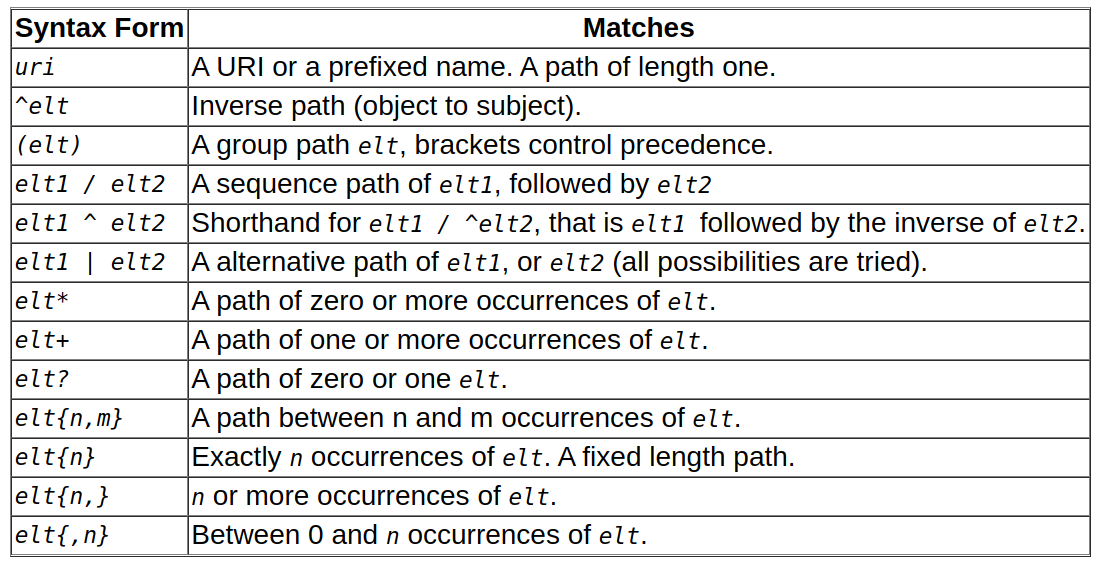
\includegraphics[width=0.8\textwidth]{pictures/pp.png}
  \caption[Property path SPARQL]{Property path SPARQL\\Sumber: \citep{sparql}}
  \label{fig:pp}
\end{figure}

Berikut adalah contoh-contoh \textit{query} SPARQL yang dilakukan pada contoh KG pada
\lst~\ref{lst:contoh-singkat-ttl}.

%--------------------------------------------------------------------------------------------------%
\subsection{Contoh Query 1}
\label{sec:contoh-query-1}
%--------------------------------------------------------------------------------------------------%

\lst~\ref{lst:query-1} merupakan SPARQL \textit{query} untuk menampilkan semua \textit{triple} yang terdapat
pada KG, akan memberikan output \tab~\ref{tab:output-query-1}. Setiap baris yang terdapat pada
output merupakan \textit{triple} yang tedapat pada KG.

\begin{listing}[H]
  \begin{minted}[fontsize=\scriptsize, frame=single]{sparql}
PREFIX ex: <https://example.org/>
SELECT ?subjek ?predikat ?objek
WHERE { ?subjek ?predikat ?objek }
  \end{minted}
  \caption{Query 1}
  \label{lst:query-1}
\end{listing}


\begin{table}
  \centering
  \begin{tabular}{|l|l|l|} \hline
    ?subjek           & ?predikat              & ?objek             \\\hline \hline
    \texttt{ex:James} & \texttt{ex:hasVisited} & \texttt{ex:Louvre} \\\hline
    \texttt{ex:James} & \texttt{ex:hasName}    & "James"            \\\hline
  \end{tabular}
  \caption{Output Query 1}
  \label{tab:output-query-1}
\end{table}

%--------------------------------------------------------------------------------------------------%
\subsection{Contoh Query 2}
\label{sec:contoh-query-2}
%--------------------------------------------------------------------------------------------------%

\lst~\ref{lst:query-2} merupakan SPARQL \textit{query} untuk menampilkan semua properti dan objek
pada \textit{triple} dengan subjek \mono{ex:James}. pada KG, akan memberikan output
\tab~\ref{tab:output-query-2}.

\begin{listing}[H]
  \begin{minted}[fontsize=\scriptsize, frame=single]{sparql}
PREFIX ex: <https://example.org/>
SELECT ?properti ?objek
WHERE { ex:James ?properti ?objek }
  \end{minted}
  \caption{Query 2}
  \label{lst:query-2}
\end{listing}

\begin{table}
  \centering
  \begin{tabular}{|l|l|} \hline
    ?properti              & ?objek             \\\hline \hline
    \texttt{ex:hasVisited} & \texttt{ex:Louvre} \\\hline
    \texttt{ex:hasName}    & "James"            \\\hline
  \end{tabular}
  \caption{Output Query 3}
  \label{tab:output-query-2}
\end{table}

%--------------------------------------------------------------------------------------------------%
\subsection{Contoh Query 3}
\label{sec:contoh-query-3}
%--------------------------------------------------------------------------------------------------%

\lst~\ref{lst:query-3} merupakan SPARQL \textit{query} untuk menampilkan semua objek pada
\textit{triple} dengan subjek \mono{ex:James} dan properti \mono{ex:hasVisited}, dengan output
\tab~\ref{tab:output-query-3}. Artinya, \textit{query} ini menampilkan semua tempat yang pernah
dikunjungi James, yaitu Louvre.

\begin{listing}[H]
  \begin{minted}[fontsize=\scriptsize, frame=single]{sparql}
PREFIX ex: <https://example.org/>
SELECT ?visited_place
WHERE { ex:James ex:hasVisited ?visited_place }
  \end{minted}
  \caption{Query 3}
  \label{lst:query-3}
\end{listing}

\begin{table}
  \centering
  \begin{tabular}{|l|l|l|} \hline
    \texttt{?visited\_place} \\ \hline \hline
    \texttt{ex:Louvre}       \\ \hline
  \end{tabular}
  \caption{Output Query 3}
  \label{tab:output-query-3}
\end{table}

%--------------------------------------------------------------------------------------------------%
\subsection{Contoh Query 4}
\label{sec:contoh-query-4}
%--------------------------------------------------------------------------------------------------%

\textit{Query} ini merupakan \textit{query} yang relatif kompleks yang akan dilakukan terhadap
\textit{server} SPARQL wikidata. Pada \textit{query} ini dilakukan pencarian artikel wikipedia dalam
dua bahasa yaitu ``en'' dan ``uz'', di mana artikelnya adalah tentang \mono{wd:Q5} yaitu manusia.

\begin{listing}[H]
  \begin{minted}[fontsize=\scriptsize, frame=single]{sparql}
SELECT DISTINCT ?lang ?name WHERE {
  ?article schema:about wd:Q5 ;
              schema:inLanguage ?lang ;
              schema:name ?name ;
              schema:isPartOf [ wikibase:wikiGroup "wikipedia" ] .
  FILTER(?lang in ('en', 'uz')) .
  \end{minted}
  \caption{Query 4}
  \label{lst:query-4}
\end{listing}

\begin{table}
  \centering
  \begin{tabular}{|l|l|} \hline
    lang & name \\ \hline \hline
    uz & Odam \\ \hline
    en & Human \\ \hline
  \end{tabular}
  \caption{Output Query 4}
  \label{tab:output-query-4}
\end{table}

%--------------------------------------------------------------------------------------------------%
\section{\Legal}
\label{sec:legal}
%--------------------------------------------------------------------------------------------------%

Menurut Pasal 7 Ayat 1 UU 10/2004 tentang pembentukan \legal, \legal adalah peraturan tertulis yang
dibentuk oleh lembaga negara atau pejabat yang berwenang dan mengikat secara umum. Jenis dan
hierarki \legal terdiri atas:

\begin{enumerate}
  \item Undang-Undang Dasar Negara Republik Indonesia Tahun 1945
  \item Undang-Undang/Peraturan Pemerintah Pengganti Undang-Undang
  \item Peraturan Pemerintah
  \item Peraturan Presiden
  \item Peraturan Daerah
\end{enumerate}

Berikut adalah beberapa peranan perundang-undangan untuk Indonesia \citep{ilmu_perundang_undangan}:

\begin{itemize}
  \item \Legal merupakan kaidah hukum yang mudah dikenal (diidentifikasi),
        mudah diketemukan kembali, dan mudah ditelusuri. Sebagai kaidah hukum tertulis, bentuk,
        jenis,dan tempatnya jelas. Begitu pula pembuatnya.
  \item \Legal memberikan kepastian hukum yang lebih nyata karena
        kaidah-kaidahnya mudah diidentifikasi dan mudah diketemukan kembali.
  \item Struktur dan sistematika \legal lebih jelas sehingga memungkinkan
        untuk diperiksa kembali dan diuji baik segi-segi formal maupun materi muatannya.
  \item Pembentukan dan pengembangan \legal dapat direncanakan. Faktor ini
        sangat penting bagi negara-negara yang sedang membangun termasuk membangun sistem hukum baru yang
        sesuai dengan kebutuhan dan perkembangan masyarakat.
\end{itemize}

Menurut lampiran UU 10/2004, struktur \legal terdiri atas:

\begin{itemize}
  \item Judul
  \item Pembukaan
  \item Batang Tubuh
  \item Penutup
  \item Penjelasan (jika diperlukan)
  \item Lampiran (jika diperlukan)
\end{itemize}

Bagian judul, pembukaan, dan penutup memuat metadata dari \legal tersebut seperti jenis, nomor,
tahun pengundangan atau penetapan, nama, jabatan pembentuk, konsiderans, kasar Hukum, \legal.
Konsiderans memuat uraian singkat mengenai pokok-pokok pikiran yang menjadi latar belakang dan
alasan pembuatan \legal. Dasar Hukum memuat dasar kewenangan pembuatan \legal dan \legal yang
memerintahkan pembuatan \legal tersebut. Oleh karena itu, kita dapat melihat keterkaitan antara
\legal dengan melihat konsiderans dan dasar hukum dari peraturan tersebut.

Batang tubuh \legal memuat semua substansi \legal yang dirumuskan dalam pasal. Pengelompokkan materi
\legal dapat disusun secara sistematis dalam buku, bab, bagian, dan paragraf atas dasar kesamaan
materi. Pasal dapat dirinci ke dalam beberapa ayat. Pasal dan ayat dapat dibuat dalam bentuk kalimat
maupun tabulasi rincian. Dalam bentuk tabulasi rincian, setiap rincian harus dapat dibaca sebagai
satu rangkaian kesatuan dengan frase pembuka dan setiap rincian diawali dengan huruf (abjad) kecil
dan diberi tanda baca titik. Suatu rincian dapat dibagi lagi ke unsur rincian yang lebih kecil.

Amendemen (perubahan) dapat dilakukan pada suatu \legal. Secara teoritis, perubahan konstitusi
(\textit{constitutional amendment}) mengandung tiga macam arti: 1) Menjadikan lain bunyi kalimatnya;
2) Menambahkan sesuatu yang baru, dan; 3) Ketentuan daman Undang-Undang Dasar dilaksanakan tidak
seperti yang tercantum di dalamnya\citep{teori_amandemen}. Bentuk amendemen dapat berupa pengubahan,
penyisipan, dan penghapusan. Amendemen juga dapat dilakukan pada tingkat peraturan maupun komponen
peraturan seperti pasal dan bab.

%--------------------------------------------------------------------------------------------------%
\section{\textit{European Legislation Identifier} (ELI)}
\label{sec:eli}
%--------------------------------------------------------------------------------------------------%

Negara-negara anggota EU memiliki cara mengatur informasi hukum yang berbeda-beda, sehingga
cenderung menghalangi penemuan, pertukaran, dan penggunaan kembali informasi. European Legislation
Identifier (ELI) adalah solusi yang bertujuan untuk mengatasi masalah-masalah tersebut. ELI
merupakan sistem untuk membuat \legal tersedia secara daring dalam format terstandardisasi, sehingga
dapat diakses dan digunakan oleh berbagai instansi \citep{eli}. ELI bertujuan untuk untuk
memfasilitasi akses, berbagi dan interkoneksi informasi hukum yang diterbitkan melalui nasional,
Eropa dan sistem informasi hukum global. ELI dibangun berdasarkan persetujuan antara negara-negara
EU.

ELI juga memiliki \textit{technical implementation
  guide}\footnote{\url{https://publications.europa.eu/en/publication-detail/-/publication/8159b75d-5efc-11e8-ab9c-01aa75ed71a1}}
yang menjelaskan implementasi ELI dan spesifikasi yang tedapat pada ELI. Spesifikasi ELI antara lain
adalah cara membuat URI suatu \textit{resource}, \textit{class}, dan properti. Ontologi yang
digunakan pada ELI cenderung untuk menjelaskan metadata dari peraturan, dan tidak memiliki pemodelan
khusus untuk menjelaskan \textit{subdivision} dari peraturan. Nyatanya, ELI menggunakan class
\textit{eli:LegalResourceSubdivision} untuk mendefinisikan semua \textit{subdivision}, tidak
terdapat kelas khusus untuk variasi \textit{subdivision} seperti bab, pasal, dan ayat. Selain itu,
ELI dirancang untuk digunakan pada peraturan di Eropa, sehingga tidak memiliki ontologi untuk jenis
peraturan di Indonesia seperti ``Peraturan Pemerintah''.

%--------------------------------------------------------------------------------------------------%
\section{Schema.org}
\label{sec:schema-org}
%--------------------------------------------------------------------------------------------------%

Schema.org adalah aktivitas komunitas kolaboratif dengan misi untuk membuat, memelihara, dan
mempromosikan skema untuk data terstruktur di internet, di halaman web, dalam pesan email, dan lebih
dari itu \citep{schema.org}. \textit{Vocabulary} Schema.org dapat digunakan dengan \textit{encoding}
yang berbeda, termasuk RDFa, Microdata dan JSON-LD. Banyak aplikasi dari Google, Microsoft,
Pinterest, Yandex, dan lainnya sudah menggunakan \textit{vocabulary} ini untuk memperkuat pengalaman
yang kaya dan dapat diperluas. Schema.org memiliki \textit{vocabulary} tersendiri untuk
\legal.\footnote{\url{https://schema.org/Legislation}} Salah satu \textit{vocabulary} nya adalah
properti yang menjelaskan metadata suatu \legal seperti \mono{legislationDate} dan
\mono{jurisdiction}.

%--------------------------------------------------------------------------------------------------%
\section{Wikidata}
\label{sec:wikidata}
%--------------------------------------------------------------------------------------------------%

Wikidata adalah basis pengetahuan \textit{free} dan terbuka yang dapat dibaca dan diedit oleh
manusia dan mesin \citep{wikidata}. Wikidata berperan sebagai penyimpanan pusat untuk data
terstruktur dari proyek saudara Wikimedia termasuk Wikipedia, Wikivoyage, Wiktionary, Wikisource,
dan lainnya. WikiProject adalah organisasi yang didirikan untuk mencapai tujuan penyuntingan
tertentu, atau untuk mencapai tujuan yang berkaitan dengan bidang pengetahuan tertentu. Terdapat
WikiProject tersendiri untuk bidang hukum dan \legal yaitu WikiProject
Law.\footnote{\url{https://www.wikidata.org/wiki/Wikidata:WikiProject_Law}} WikiProject Law
menyediakan properti terkait \legal sebagaimana yang dapat dilihat pada \pic~\ref{fig:wikiproject}
dan beberapa deskripsinya pada \tab~\ref{tab:wp-desc}.

\begin{figure}[H]
  \centering
  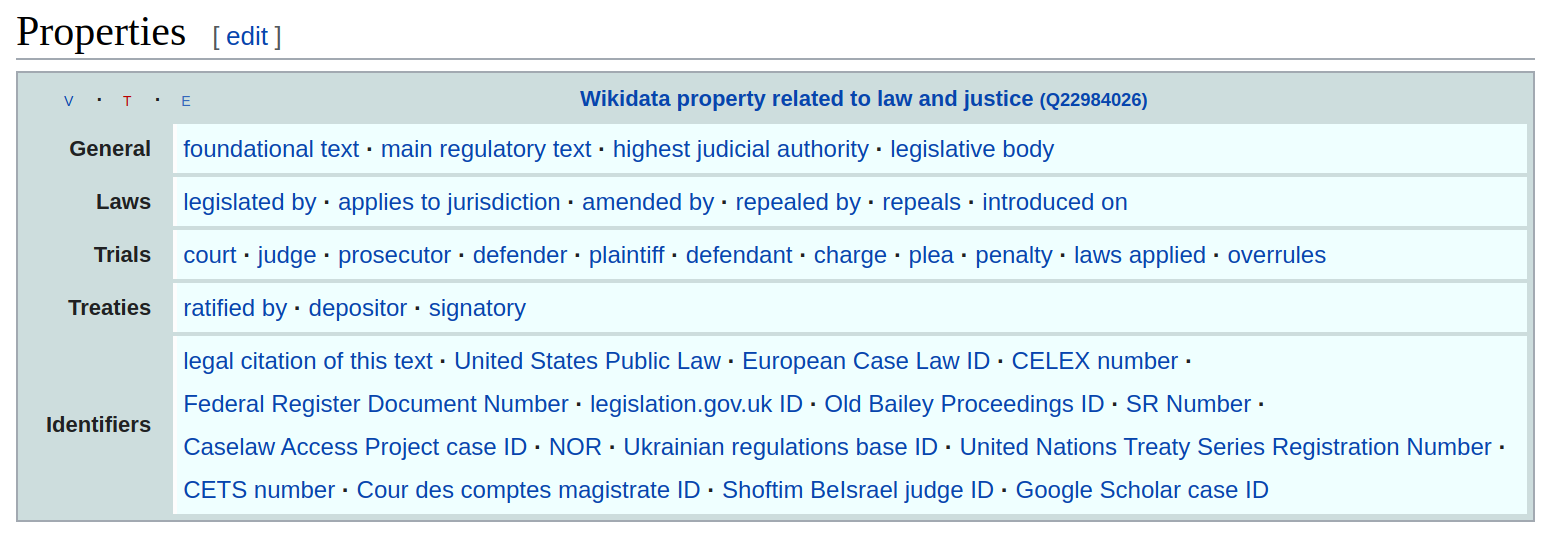
\includegraphics[width=0.8\textwidth]{pictures/wikiproject.png}
  \caption{Properti WikiProject Law}
  \label{fig:wikiproject}
\end{figure}

\begin{table}
  \centering
  \begin{tabular}{|p{0.2\textwidth}|p{0.8\textwidth}|} \hline
    label                   & deskripsi                                                                                                                                                                                          \\\hline \hline
    amended by              & document is amended by specified other document                                                                                                                                                    \\\hline
    legislated by           & indicates that an act or bill was passed by a legislature. The value can be a particular session of the legislature                                                                                \\\hline
    applies to jurisdiction & the item (institution, law, public office, public register...) or statement belongs to or has power over or applies to the value (a territorial jurisdiction: a country, state, municipality, ...) \\\hline
  \end{tabular}
  \caption{Deskripsi beberapa Properti WikiProject Law}
  \label{tab:wp-desc}
\end{table}

